\documentclass[tikz,border=5pt]{standalone}
\usepackage[utf8]{inputenc}
\usepackage[T1]{fontenc}
\usepackage{amsmath,amssymb}
\usepackage{lmodern}
\usetikzlibrary{arrows.meta}

\definecolor{ink}{HTML}{1d1d1f}
\definecolor{graytext}{HTML}{515154}
\definecolor{muted}{HTML}{86868b}
\definecolor{linegray}{HTML}{d2d2d7}
\definecolor{mistbg}{HTML}{f5f5f7}
\definecolor{blueaccent}{HTML}{2997ff}
\definecolor{bluedark}{HTML}{0066cc}
\definecolor{amber}{HTML}{ff9f0a}
\definecolor{amberdark}{HTML}{c76008}
\definecolor{greendark}{HTML}{1a7f37}
\definecolor{greenaccent}{HTML}{30d158}
\definecolor{redaccent}{HTML}{ff453a}
\definecolor{reddark}{HTML}{d70015}

\begin{document}
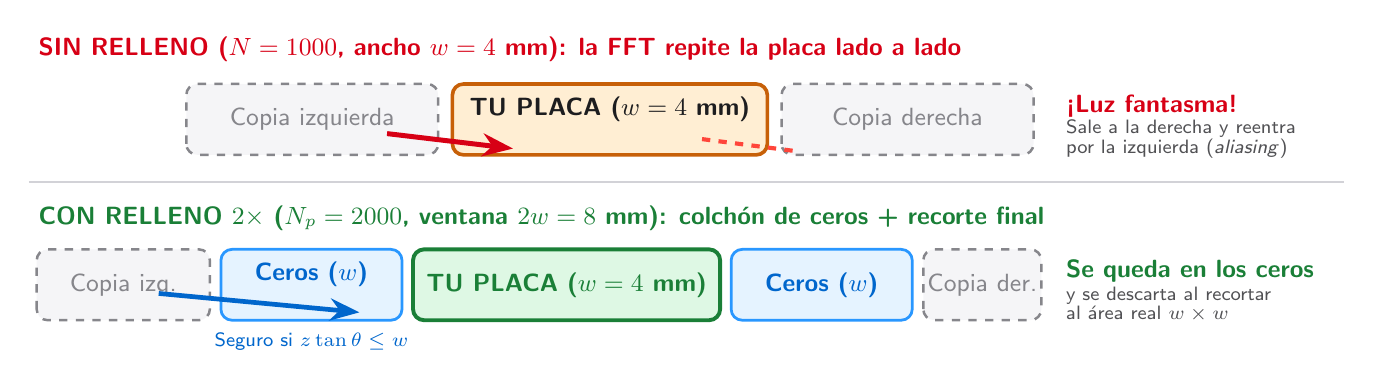
\begin{tikzpicture}[font=\sffamily,>=Stealth]

% --- Fila 1: Sin relleno ---
\node[anchor=west,font=\sffamily\bfseries\small,text=reddark] at (0,3.92)
  {SIN RELLENO ($N = 1000$, ancho $w = 4\text{ mm}$): la FFT repite la placa lado a lado};

\draw[dashed,muted,fill=mistbg,rounded corners=4pt,line width=0.9pt] (2.0,2.58) rectangle (5.2,3.48);
\node[text=muted,font=\sffamily\small] at (3.6,3.03) {Copia izquierda};

\draw[amberdark,fill=amber!18,rounded corners=4pt,line width=1.3pt] (5.38,2.58) rectangle (9.38,3.48);
\node[text=ink,font=\sffamily\bfseries\small] at (7.38,3.16) {TU PLACA ($w = 4\text{ mm}$)};

\draw[dashed,muted,fill=mistbg,rounded corners=4pt,line width=0.9pt] (9.56,2.58) rectangle (12.76,3.48);
\node[text=muted,font=\sffamily\small] at (11.16,3.03) {Copia derecha};

% Rayos Pac-Man en franja inferior del bloque para no pisar el texto
\draw[redaccent,line width=1.5pt,dashed] (8.55,2.78) -- (9.80,2.62);
\draw[->,reddark,line width=1.8pt] (4.55,2.85) -- (6.15,2.66);

\node[anchor=west,text=reddark,font=\sffamily\bfseries\small] at (13.05,3.20) {¡Luz fantasma!};
\node[anchor=west,text=graytext,font=\sffamily\scriptsize,align=left] at (13.05,2.78) {Sale a la derecha y reentra\\[-1pt]por la izquierda (\emph{aliasing})};

% Separador
\draw[linegray,line width=0.8pt] (0,2.24) -- (16.7,2.24);

% --- Fila 2: Con relleno 2x ---
\node[anchor=west,font=\sffamily\bfseries\small,text=greendark] at (0,1.78)
  {CON RELLENO $2\times$ ($N_p = 2000$, ventana $2w = 8\text{ mm}$): colchón de ceros + recorte final};

\draw[dashed,muted,fill=mistbg,rounded corners=4pt,line width=0.9pt] (0.10,0.48) rectangle (2.30,1.38);
\node[text=muted,font=\sffamily\small] at (1.20,0.93) {Copia izq.};

\draw[blueaccent,fill=blueaccent!12,rounded corners=4pt,line width=1.0pt] (2.44,0.48) rectangle (4.74,1.38);
\node[text=bluedark,font=\sffamily\bfseries\small] at (3.59,1.06) {Ceros ($w$)};

\draw[greendark,fill=greenaccent!16,rounded corners=4pt,line width=1.4pt] (4.88,0.48) rectangle (8.78,1.38);
\node[text=greendark,font=\sffamily\bfseries\small] at (6.83,0.93) {TU PLACA ($w = 4\text{ mm}$)};

\draw[blueaccent,fill=blueaccent!12,rounded corners=4pt,line width=1.0pt] (8.92,0.48) rectangle (11.22,1.38);
\node[text=bluedark,font=\sffamily\bfseries\small] at (10.07,0.93) {Ceros ($w$)};

\draw[dashed,muted,fill=mistbg,rounded corners=4pt,line width=0.9pt] (11.36,0.48) rectangle (12.86,1.38);
\node[text=muted,font=\sffamily\small] at (12.11,0.93) {Copia der.};

% Rayo cayendo en la parte inferior de Ceros (w)
\draw[->,bluedark,line width=1.7pt] (1.65,0.82) -- (4.20,0.58);
\node[anchor=north,text=bluedark,font=\sffamily\scriptsize] at (3.59,0.44) {Seguro si $z\tan\theta \le w$};

\node[anchor=west,text=greendark,font=\sffamily\bfseries\small] at (13.05,1.10) {Se queda en los ceros};
\node[anchor=west,text=graytext,font=\sffamily\scriptsize,align=left] at (13.05,0.68) {y se descarta al recortar\\[-1pt]al área real $w \times w$};

\end{tikzpicture}
\end{document}
